% figures-es/channel-structure.tex
% Standalone TikZ: estructura de canal — cadenas de canal directo, de un nivel y de dos niveles (ch.10).
\documentclass[tikz,border=6pt]{standalone}
\usepackage{tikz}
\usetikzlibrary{arrows.meta,positioning,calc}

\definecolor{vcblue}{HTML}{1A5276}
\definecolor{vcteal}{HTML}{0E6655}
\definecolor{vcgrey}{HTML}{5D6D7E}

\begin{document}
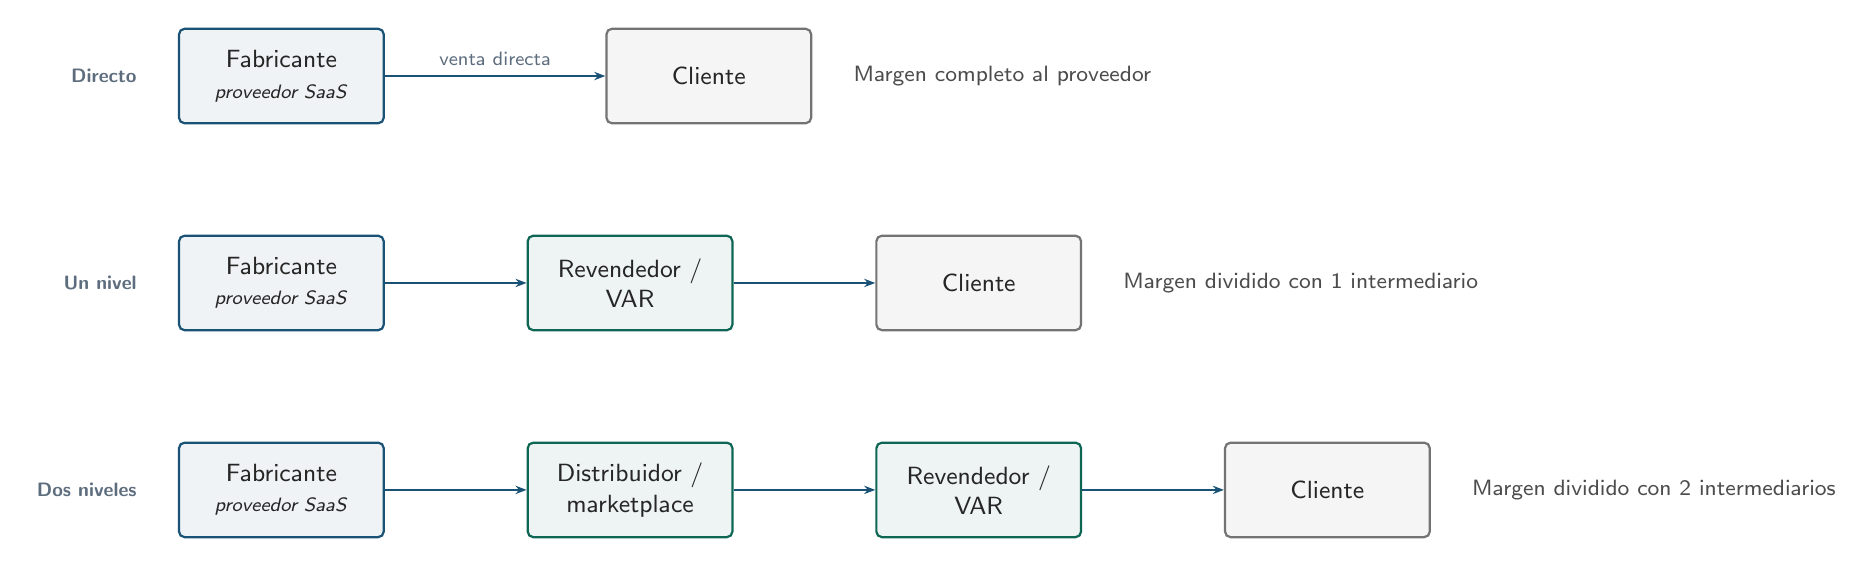
\begin{tikzpicture}[
  node distance=6mm,
  box/.style={draw=vcblue, line width=0.8pt, rounded corners=2pt, fill=vcblue!7,
              font=\sffamily\small, align=center,
              minimum width=26mm, minimum height=12mm, text=black!85},
  interm/.style={draw=vcteal, line width=0.8pt, rounded corners=2pt, fill=vcteal!7,
                 font=\sffamily\small, align=center,
                 minimum width=26mm, minimum height=12mm, text=black!85},
  cust/.style={draw=black!55, line width=0.8pt, rounded corners=2pt, fill=black!4,
               font=\sffamily\small, align=center,
               minimum width=26mm, minimum height=12mm, text=black!85},
  arrow/.style={-{Stealth[length=4pt]}, vcblue, line width=0.9pt},
  lbl/.style={font=\sffamily\scriptsize\bfseries, text=vcgrey, align=left},
  row/.style={font=\sffamily\footnotesize, text=black!70, align=left},
]

%% ---- Fila 1: canal directo ----
\node[box]  (m1) {Fabricante\\{\scriptsize\textit{proveedor SaaS}}};
\node[cust, right=28mm of m1] (c1) {Cliente};

\draw[arrow] (m1.east) -- node[above,font=\sffamily\scriptsize,text=vcgrey]{venta directa} (c1.west);

%% ---- Fila 2: canal de un nivel ----
\node[box,  below=14mm of m1]  (m2) {Fabricante\\{\scriptsize\textit{proveedor SaaS}}};
\node[interm, right=18mm of m2] (r2) {Revendedor /\\VAR};
\node[cust, right=18mm of r2]  (c2) {Cliente};

\draw[arrow] (m2.east) -- (r2.west);
\draw[arrow] (r2.east) -- (c2.west);

%% ---- Fila 3: canal de dos niveles ----
\node[box,  below=14mm of m2]  (m3) {Fabricante\\{\scriptsize\textit{proveedor SaaS}}};
\node[interm, right=18mm of m3] (d3) {Distribuidor /\\marketplace};
\node[interm, right=18mm of d3] (r3) {Revendedor /\\VAR};
\node[cust, right=18mm of r3]  (c3) {Cliente};

\draw[arrow] (m3.east) -- (d3.west);
\draw[arrow] (d3.east) -- (r3.west);
\draw[arrow] (r3.east) -- (c3.west);

%% ---- Etiquetas de fila en el margen izquierdo ----
\node[lbl, left=4mm of m1] {Directo};
\node[lbl, left=4mm of m2] {Un nivel};
\node[lbl, left=4mm of m3] {Dos niveles};

%% ---- Anotaciones de margen (a la derecha de los nodos de cliente) ----
\node[row, right=4mm of c1] {Margen completo al proveedor};
\node[row, right=4mm of c2] {Margen dividido con 1 intermediario};
\node[row, right=4mm of c3] {Margen dividido con 2 intermediarios};

\end{tikzpicture}
\end{document}
